\documentclass[oneside,numbers,spanish]{ezthesis}
%% # Opciones disponibles para el documento #
%%
%% Las opciones con un (*) son las opciones predeterminadas.
%%
%% Modo de compilar:
%%   draft            - borrador con marcas de fecha y sin im'agenes
%%   draftmarks       - borrador con marcas de fecha y con im'agenes
%%   final (*)        - version final de la tesis
%%
%% Tama'no de papel:
%%   letterpaper (*)  - tama'no carta (Am'erica)
%%   a4paper          - tama'no A4    (Europa)
%%
%% Formato de impresi'on:
%%   oneside          - hojas impresas por un solo lado
%%   twoside (*)      - hijas impresas por ambos lados
%%
%% Tama'no de letra:
%%   10pt, 11pt, o 12pt (*)
%%
%% Espaciado entre renglones:
%%   singlespace      - espacio sencillo
%%   onehalfspace (*) - espacio de 1.5
%%   doublespace      - a doble espacio
%%
%% Formato de las referencias bibliogr'aficas:
%%   numbers          - numeradas, p.e. [1]
%%   authoryear (*)   - por autor y a'no, p.e. (Newton, 1997)
%%
%% Opciones adicionales:
%%   spanish         - tesis escrita en espa'nol
%%
%% Desactivar opciones especiales:
%%   nobibtoc   - no incluir la bibiolgraf'ia en el 'Indice general
%%   nofancyhdr - no incluir "fancyhdr" para producir los encabezados
%%   nocolors   - no incluir "xcolor" para producir ligas con colores
%%   nographicx - no incluir "graphicx" para insertar gr'aficos
%%   nonatbib   - no incluir "natbib" para administrar la bibliograf'ia

%% Paquetes adicionales requeridos se pueden agregar tambi'en aqu'i.
%% Por ejemplo:
%\usepackage{subfig}
%\usepackage{multirow}
\usepackage{float}
%\floatstyle{boxed} 
\restylefloat{figure}
\usepackage{graphicx}
\usepackage{caption}

\usepackage[utf8]{inputenc}
\usepackage{ragged2e} %justify text

\usepackage{lipsum}%citas palabras de un personaje en el centro
\usepackage{clipboard}%citas palabras de un personaje en el centro

%\usepackage{apacite}
%\usepackage{cite}


%% # Datos del documento #
%% Nota que los acentos se deben escribir: \'a, \'e, \'i, etc.
%% La letra n con tilde es: \~n.

\author{David Guillermo L\'opez V\'azquez}
\title{CLASIFICADOR ESTADÍSTICO PARA LA PREVENCIÓN Y AUXILIO EN POTENCIALES CASOS DE FEMINICIDIO}
\degree{Ingeniero en Ciencias Computacionales}
\supervisor{Nombre de mi Asesor}
\institution{Benem\'erita Universidad Aut\'onoma de Puebla}
\faculty{Facultad de Ciencias de la Computaci\'on}
\department{Departamento de Sistemas Computacionales}

%% # M'argenes del documento #
%% 
%% Quitar el comentario en la siguiente linea para austar los m'argenes del
%% documento. Leer la documentaci'on de "geometry" para m'as informaci'on.

%\geometry{top=40mm,bottom=33mm,inner=40mm,outer=25mm}

%% El siguiente comando agrega ligas activas en el documento para las
%% referencias cruzadas y citas bibliogr'aficas. Tiene que ser *la 'ultima*
%% instrucci'on antes de \begin{document}.
\hyperlinking
\begin{document}

%% En esta secci'on se describe la estructura del documento de la tesis.
%% Consulta los reglamentos de tu universidad para determinar el orden
%% y la cantidad de secciones que debes de incluir.

%% # Portada de la tesis #
%% Mirar el archivo "titlepage.tex" para los detalles.
%% ## Construye tu propia portada ##
%% 
%% Una portada se conforma por una secuencia de "Blocks" que incluyen
%% piezas individuales de informaci'on. Un "Block" puede incluir, por
%% ejemplo, el t'itulo del documento, una im'agen (logotipo de la universidad),
%% el nombre del autor, nombre del supervisor, u cualquier otra pieza de
%% informaci'on.
%%
%% Cada "Block" aparece centrado horizontalmente en la p'agina y,
%% verticalmente, todos los "Blocks" se distruyen de manera uniforme 
%% a lo largo de p'agina.
%%
%% Nota tambi'en que, dentro de un mismo "Block" se pueden cortar
%% lineas usando el comando \\
%%
%% El tama'no del texto dentro de un "Block" se puede modificar usando uno de
%% los comandos:
%%   \small      \LARGE
%%   \large      \huge
%%   \Large      \Huge
%%
%% Y el tipo de letra se puede modificar usando:
%%   \bfseries - negritas
%%   \itshape  - it'alicas
%%   \scshape  - small caps
%%   \slshape  - slanted
%%   \sffamily - sans serif
%%
%% Para producir plantillas generales, la informaci'on que ha sido inclu'ida
%% en el archivo principal "tesis.tex" se puede accesar aqu'i usando:
%%   \insertauthor
%%   \inserttitle
%%   \insertsupervisor
%%   \insertinstitution
%%   \insertdegree
%%   \insertfaculty
%%   \insertdepartment
%%   \insertsubmitdate

\begin{titlepage}
  \TitleBlock{\scshape\insertinstitution}
  \TitleBlock[\bigskip]{\scshape\insertfaculty}
  \TitleBlock{\Huge\scshape\inserttitle}
  \TitleBlock{\scshape
    Tesis presentada por \insertauthor \\
    para obtener el grado de \insertdegree}
  \TitleBlock{\insertsubmitdate}
  \TitleBlock[\bigskip]{\insertdepartment}
\end{titlepage}

%% Nota 1:
%% Se puede agregar un escudo o logotipo en un "Block" como:
%%   \TitleBlock{\includegraphics[height=4cm]{escudo_uni}}
%% y teniendo un archivo "escudo_uni.pdf", "escudo_uni.png" o "escudo_uni.jpg"
%% en alg'un lugar donde LaTeX lo pueda encontrar.

%% Nota 2:
%% Normalmente, el espacio entre "Blocks" se extiende de modo que el
%% contenido se reparte uniformemente sobre toda la p'agina. Este
%% comportamiento se puede modificar para mantener fijo, por ejemplo, el
%% espacio entre un par de "Blocks". Escribiendo:
%%   \TitleBlock{Bloque 1}
%%   \TitleBlock[\bigskip]{Bloque2}
%% se deja un espacio "grande" y de tama~no fijo entre el bloque 1 y 2.
%% Adem'as de \bigskip est'an tambi'en \smallskip y \medskip. Si necesitas
%% aun m'as control puedes usar tambi'en, por ejemplo, \vspace*{2cm}.




%% # Prefacios #
%% Por cada prefacio (p.e. agradecimientos, resumen, etc.) crear
%% un nuevo archivo e incluirlo aqu'i.
%% Para m'as detalles y un ejemplo mirar el archivo "gracias.tex".
%% Las secciones del "prefacio" inician con el comando \prefacesection{T'itulo}
%% Este tipo de secciones *no* van numeradas, pero s'i aparecen en el 'indice.
%%
%% Si quieres agregar una secci'on que no vaya n'umerada y que *tampoco*
%% aparesca en el 'indice, usa entonces el comando \chapter*{T'itulo}
%%
%% Recuerda que aqu'i ya puedes escribir acentos como: 'a, 'e, 'i, etc.
%% La letra n con tilde es: 'n.

\prefacesection{Agradecimientos}

Este trabajo no habr'ia sido posible sin el apoyo y el est'imulo de mi colega
y amigo, Doctor Rudolf Fliesning,  bajo cuya supervisi'on escog'i este tema y
comenc'e la tesis. Sr. Quentin Travers, mi consejero en las etapas finales
del trabajo, tambi'en ha sido generosamente servicial, y me ha ayudado de
numerosos modos, incluyendo el resumen del contenido de los documentos que
no estaban disponibles para mi examen, y en particular por permitirme leer, 
en cuanto estuvieron  disponibles, las copias de los  recientes extractos de
los diarios de campa'na del Vigilante Rupert Giles y la actual Cazadora la
se'norita Buffy Summers, que se encontraron con William the Bloody en 1998, y
por facilitarme el pleno acceso  a los diarios de anteriores Vigilantes
relevantes a la carrera de William the Bloody.

Tambi'en me gustar'ia agradecerle al Consejo la concesi'on de Wyndham-Pryce
como Compa'nero, el cual me ha apoyado durante mis dos a'nos de investigaci'on,
y la concesi'on de dos subvenciones de viajes, una para estudiar documentos
en los Archivos de Vigilantes sellados en Munich, y otra para la
investigaci'on en campa'na en Praga. Me gustar'ia agradecer a Sr. Travers,
otra vez, por facilitarme  la acreditaci'on  de seguridad para el trabajo en
los Archivos de Munich, y al Doctor Fliesning por su apoyo colegial y ayuda
en ambos viajes de investigaci'on.

No puedo terminar sin agradecer a mi familia, en cuyo est'imulo constante y
amor he confiado a lo largo de mis a'nos en la Academia. Estoy agradecida
tambi'en a los ejemplos de mis  difuntos hermano, Desmond Chalmers, Vigilante
en Entrenamiento, y padre, Albert Chalmers, Vigilante. Su coraje resuelto
y convicci'on siempre me inspirar'an, y espero seguir, a mi propio y peque'no
modo, la noble misi'on por la que dieron sus vidas. Es a ellos a quien dedico
este trabajo.

%% Por si alguien tiene curiosidad, este "simp'atico" agradecimiento est'a
%% tomado de la "Tesis de Lydia Chalmers" basada en el universo del programa
%% de televisi'on Buffy, la Cazadora de Vampiros.
%% http://www.buffy-cazavampiros.com/Spiketesis/tesis.inicio.htm


%% # 'Indices y listas de contenido #
%% Quitar los comentarios en las lineas siguientes para obtener listas de
%% figuras y cuadros/tablas.
\tableofcontents
%\listoffigures
%\listoftables

%% # Cap'itulos #
%% Por cada cap'itulo hay que crear un nuevo archivo e incluirlo aqu'i.
%% Mirar el archivo "intro.tex" para un ejemplo y recomendaciones para
%% escribir.
%% Los cap'itulos inician con \chapter{T'itulo}, estos aparecen numerados y
%% se incluyen en el 'indice general.
%%
%% Recuerda que aqu'i ya puedes escribir acentos como: 'a, 'e, 'i, etc.
%% La letra n con tilde es: 'n.

\chapter{Introducci'on}

Actualmente la difusión de la tecnología ubicua sobre todo la móvil se ha extendido ampliamente gracias al uso del internet y los telefonos inteligentes o smartphones,  así la disminución de costos de los mismos. Lo anterior nos da un ecosistema fertil para un desarrollar un sin fin de aplicativos.

Cabe especificar que los smartphones cuentan con diversos sensores integrados, como lo son: acelerómetros, giroscopio, sensor de huella, sensor dactilar, bluethoot, magnetómetro, receptor GPS, etc. Y es precismente este último el que nos interesa para nuestro desarrollo.

El receptor GPS se encarga de obtener la ubicación exacta con errores mínimos pudiendonos dar: la latitud, longitud y altitud del dispositivo. Apartir de éstos datos podemos obtener información diversa como: la velocidad de desplazamiento del dispositivo, la hora exacta del dispositivo en base a su posición, la distancia a un punto dado al dispositivo, si el dispositivo ha entrado a un área en especifica, si ha salido de un área en específica. 

Con este conocimiento y la violencia e inseguridad que actualmente sufre México, buscamos que la tecnología se vuelva una aliada en el rastreo de personas, especificamente enfrentar el problema de "feminicidios" en el estado de Puebla. 

Para que las familias y seres queridos de estas personas tengan en medida de lo posible, la tranquilidad de conocer su paradero y saber que se encuentra bien y a salvo.

\chapter{Objetivos}

\begin{itemize}
\item \textbf{Objetivos Generales}\itemsep2pt\\
\begin{description}
%\item \textbf{Objetivos Generales}\\
% \par\rlap{Here the text is using the full text width ignoring the list indent.}
Desarrollar una aplicación ubicua que permita monitorear y rastrear personas del sexo femenino en el estado de Puebla.
\end{description}
\item \textbf{Objetivos Especificos}\itemsep2pt\\
\begin{enumerate}
%\item \textbf{Objetivos Generales}\\
% \par\rlap{Here the text is using the full text width ignoring the list indent.}
\item Montar un servidor.
\item Montar Base Datos.
\item Instalar un API Rest con CRUD a la DB.
\item Conectar un dispositivo de rastreo al API Rest.
\item Desarrollar una capa de consumo de servicios REST.
\item Mostrar en tiempo real la última ubicación.
\item Mostrar un historial por fecha indicada de ubicación.
\item Notificación sale del perímetro.
\end{enumerate}
\end{itemize}






\chapter{Planteamiento del problema}

\subsection{Desaparici\'on forzada de personas en México}

\justify
La desaparición forzada de personas en México es una problematica social que se ha encrudeció en años recientes. El Registro Nacional de Datos de Personas Extraviadas o Desaparecidas (RNPED), integra los datos de personas no localizadas en México. Obtenidos a partir de las denuncias presentadas ante la autoridad ministerial correspondiente. Este registro incluye únicamente a las personas que a la fecha de corte, continuan sin ser localizadas.



%\begin{figure}
%  \caption{A picture of a gull.}
%  \centering
%    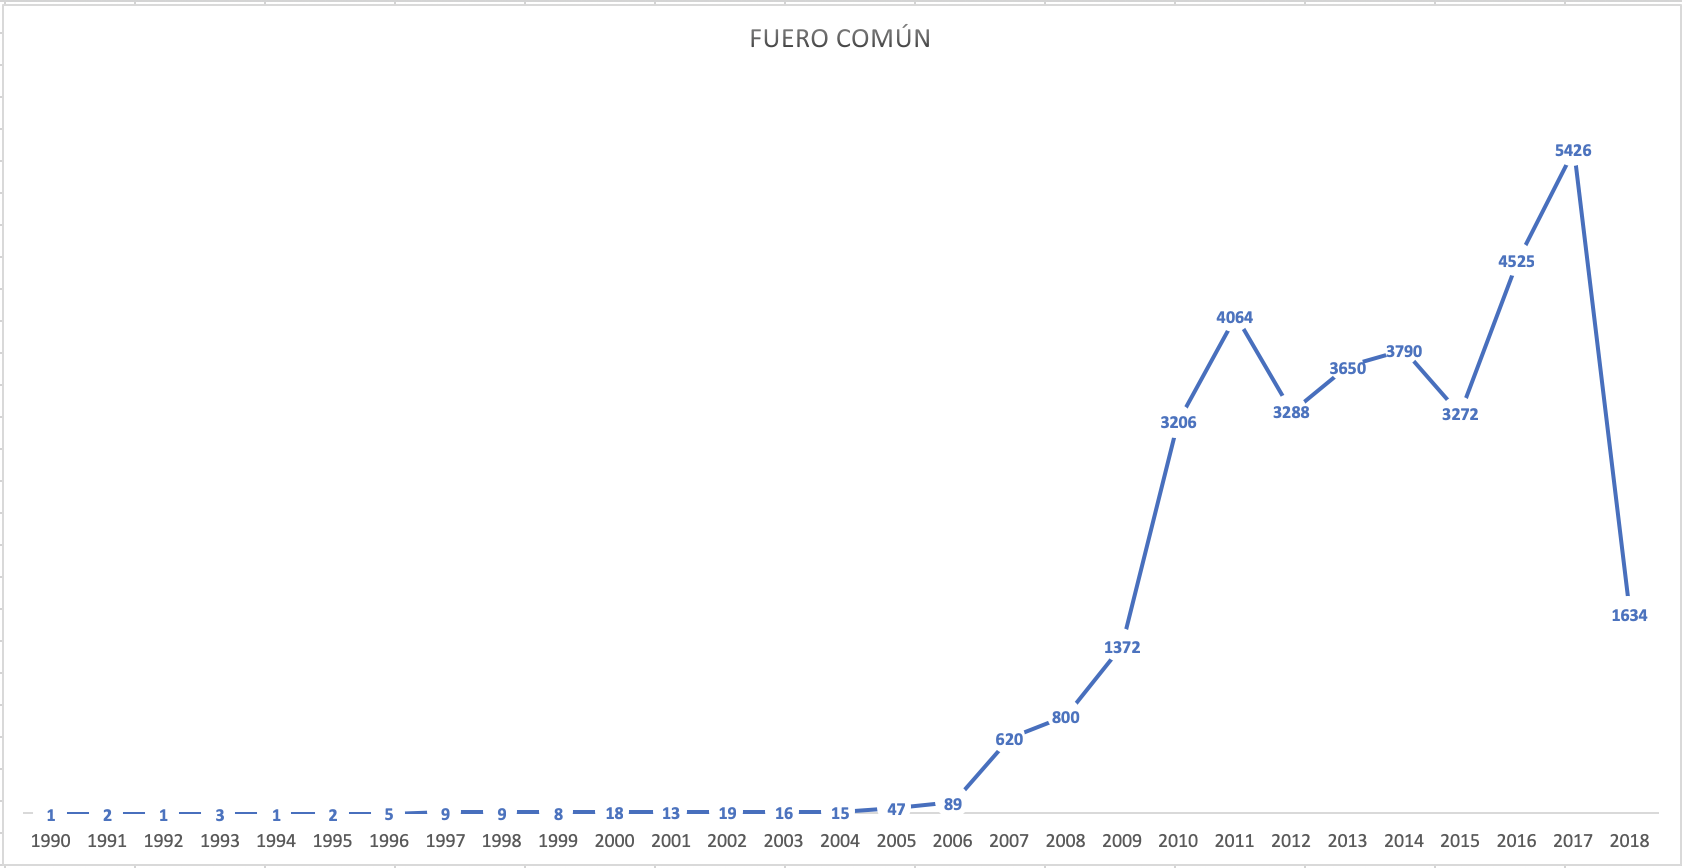
\includegraphics[width=0.5\textwidth]{imgs/fuerocomun}
%\end{figure}

%\begin{figure}
%  \centering 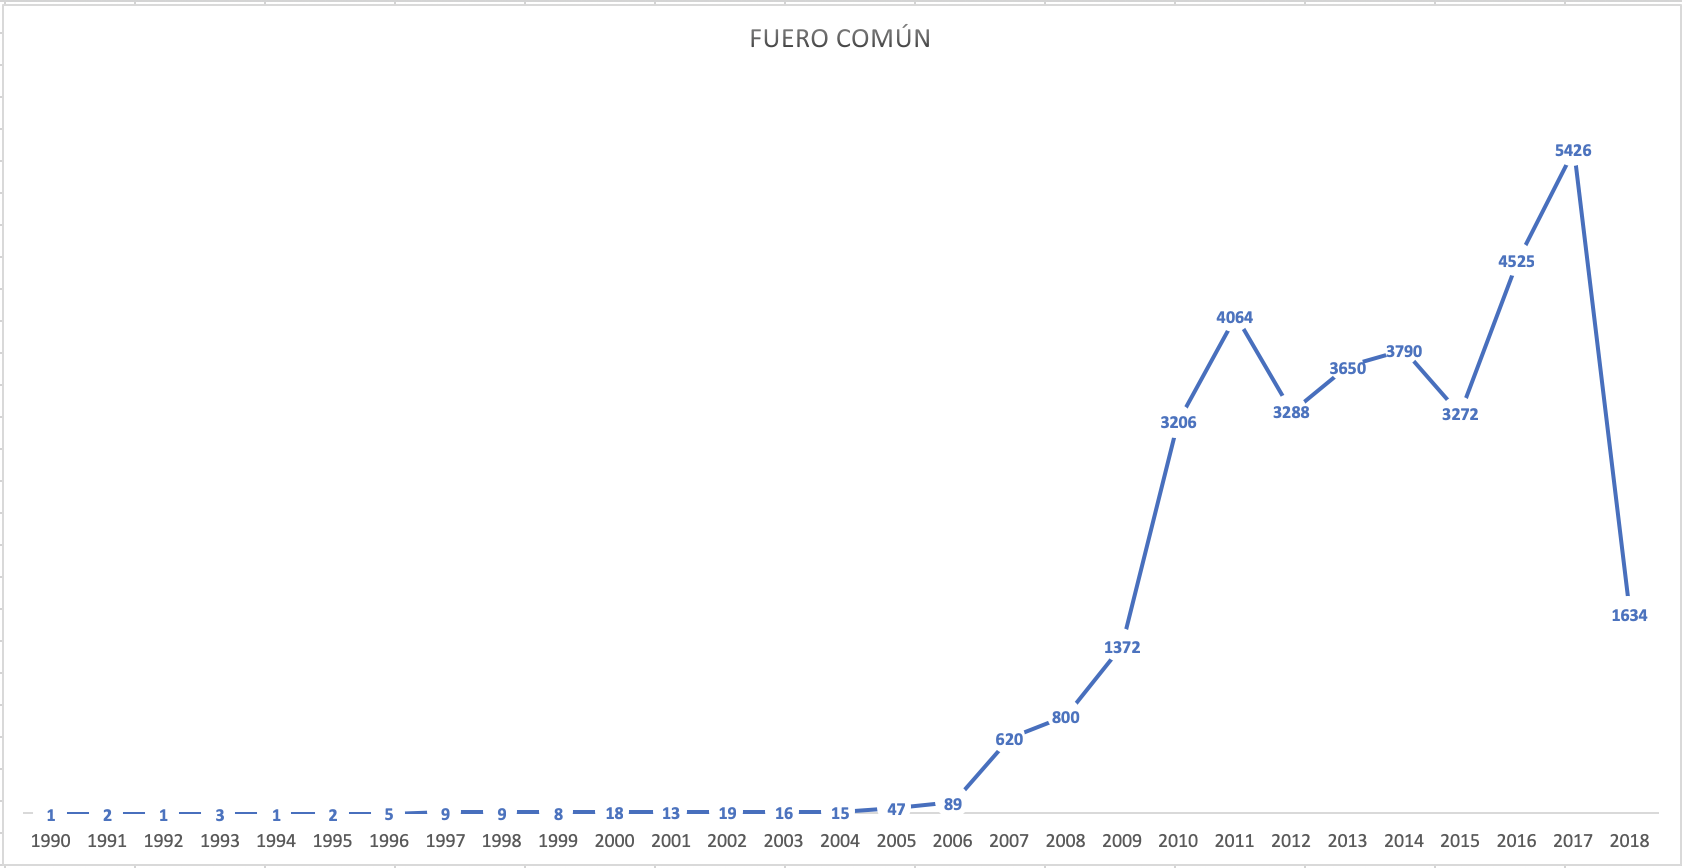
\includegraphics[width=0.3\linewidth]{imgs/fuerocomun.png} \qquad
%  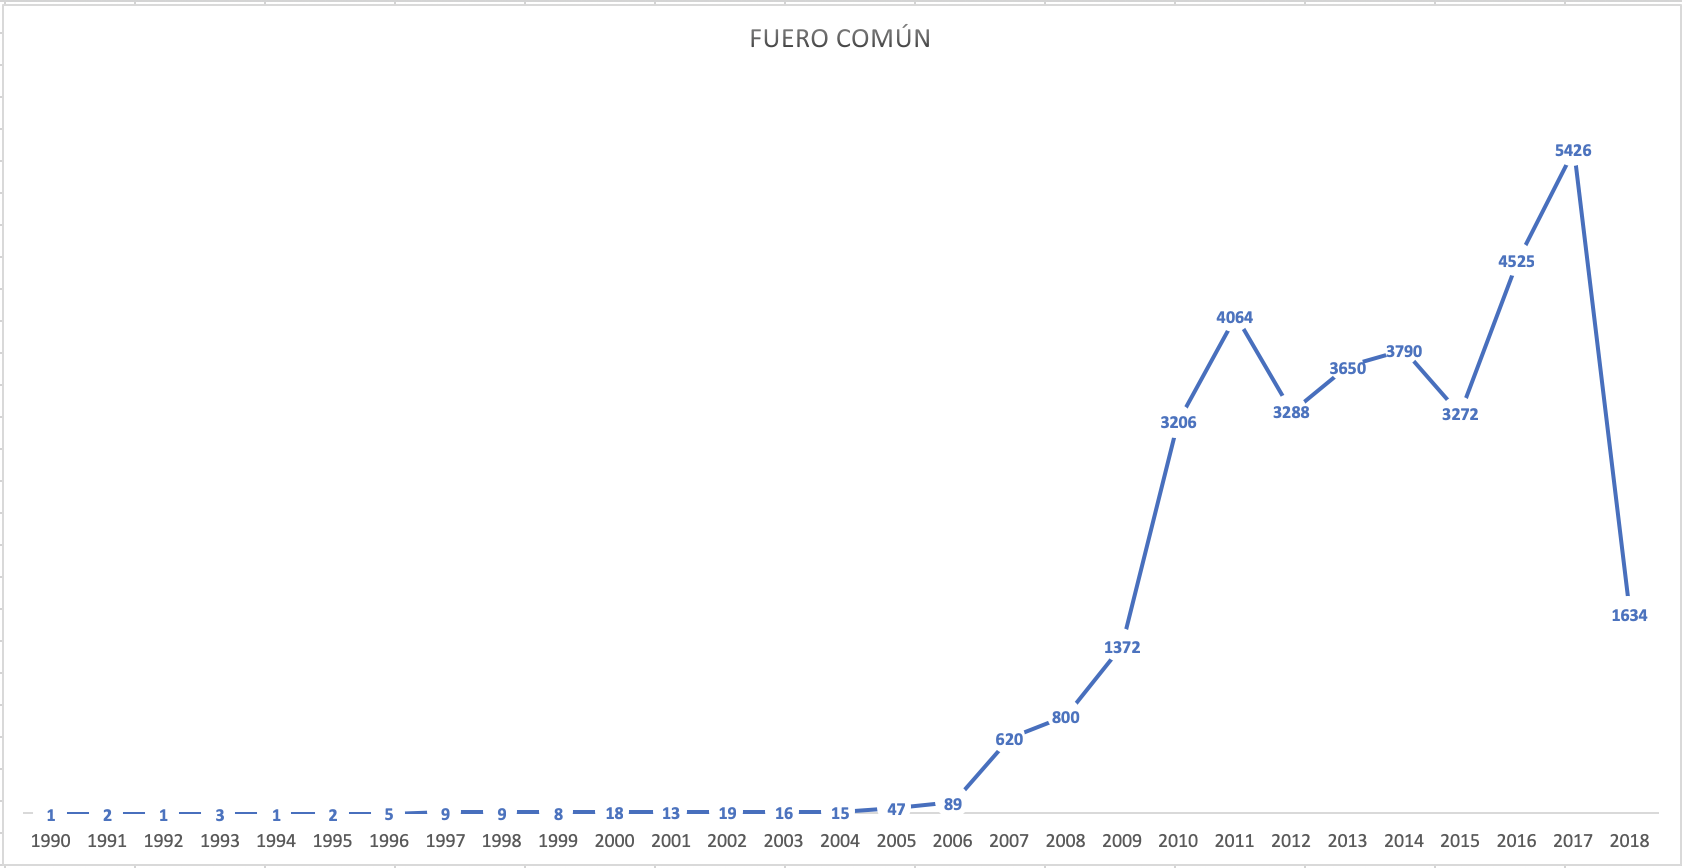
\includegraphics[width=0.3\linewidth]{imgs/fuerocomun.png}
%  \caption{Diagram from Patent Application 12/475,048}
%\end{figure}

\begin{figure}[bp!]
	\centering
	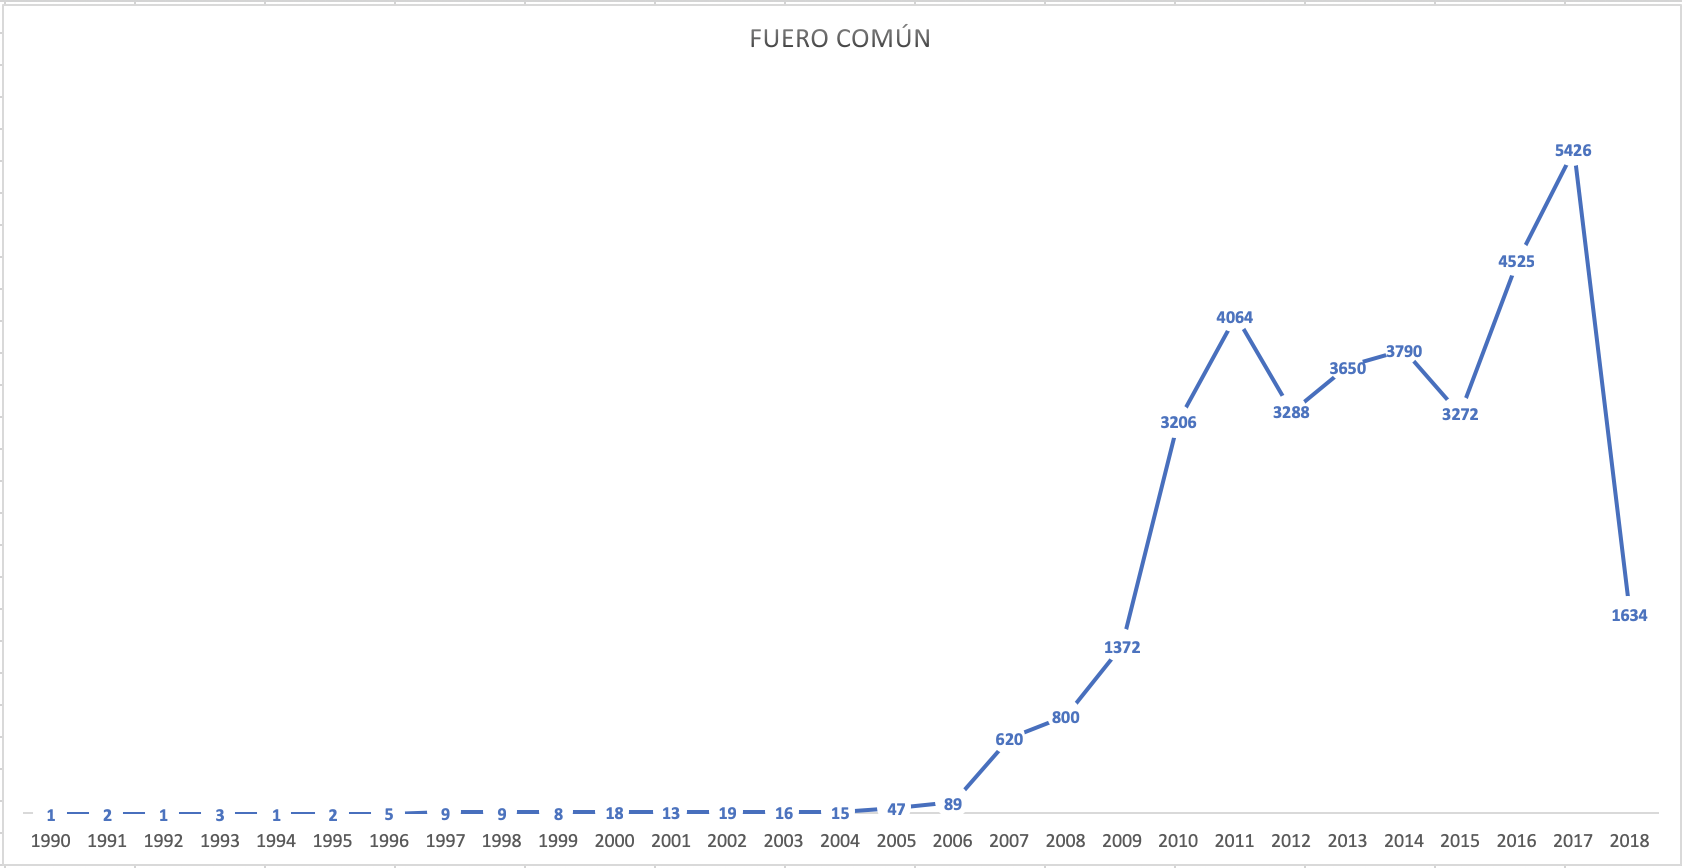
\includegraphics[width=5in]{imgs/fuerocomun}
	  \caption{Estad\'istica Fuero Común}
\end{figure}

\begin{figure}[bp!]
	\centering
	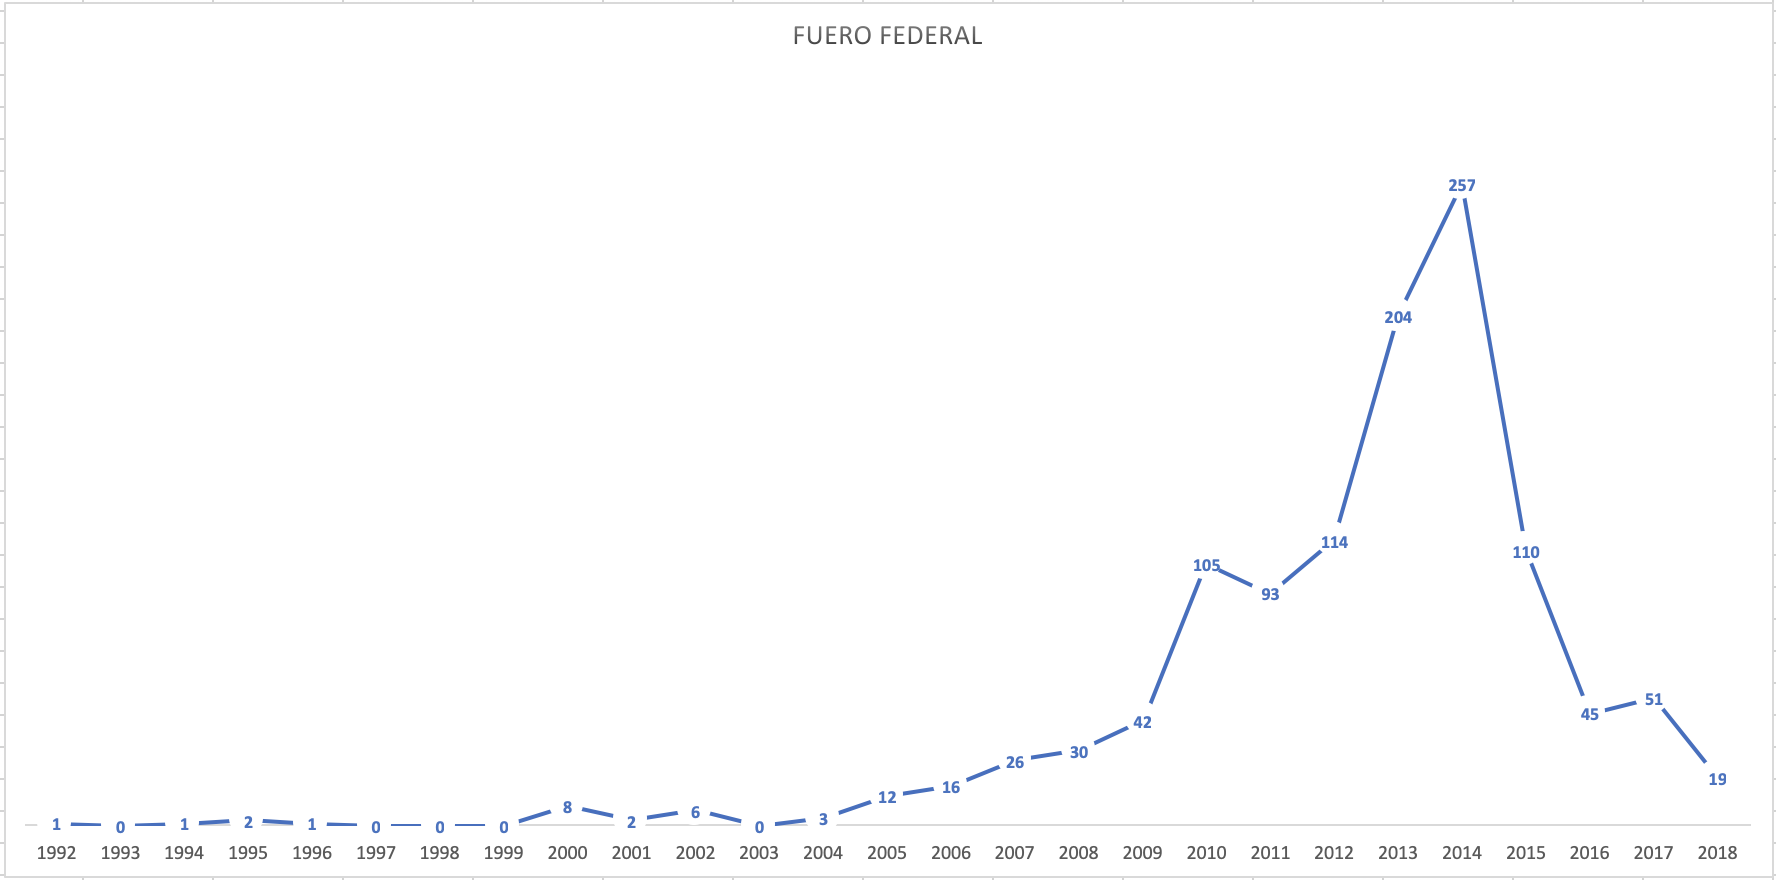
\includegraphics[width=5in]{imgs/fuerofederal}
	  \caption{Estad\'istica Fuero Federal}
\end{figure}


\justify
Se entiende por persona desaparecida a toda aquella que, con base en información fidedigna de familiares, personas cercanas o vinculadas a ella, se le haya dado por desaparecida, en conformidad con el derecho internacional, lo cual puede estar relacionado con: un conflicto armado internacional o no internacional, una situación de violencia o disturbios de carácter interno, una catástrofe natural o cualquier situación que pudiera requerir la intervención de una autoridad pública competente.


\begin{flushleft}
El RNPED se divide en Fuero Com\'un y Fuero Federal.
\end{flushleft}

\paragraph{Fuero Com\'un}
Y cuando se hace referencia al fuero com\'un o local, se hace referencia a la aplicación territorial de las leyes locales, de las entidades federativas. Como el Código Penal del Distrito Federal, Código Civil del Distrito Federal, etc.

\paragraph{Fuero Federal}
En concreto fuero federal se refiere a la correspondencia de aplicación de leyes federales, en un caso concreto a delitos cometidos en territorio que se considera federal o delitos que se encuentran tipificados en los ordenamientos federales como el Código Federal de Procedimientos Penales, como la Ley de Amparo, la Ley Agraria, etc.

%\begin{flushleft}
%Aun que en 2018 se ve disminuido, estos datos se ven influenciados debido a que el RNPED realizo su fecha de corte el 30 de abril por motivos de delegar esta tarea a a la Comisión Nacional de Búsqueda de Personas como lo informan en su página:
%
%Se informa que el Secretariado Ejecutivo del Sistema Nacional de Seguridad Pública realizó por última ocasión la actualización de las bases de datos del Registro Nacional de Datos de Personas Extraviadas o Desaparecidas (RNPD) del fuero común y fuero federal con corte al 30 de abril.
%
%Cabe mencionar que corresponderá a la Comisión Nacional de Búsqueda de Personas la publicación de las subsecuentes bases de datos, de conformidad con la Ley General en materia de Desaparición Forzada de Personas, Desaparición cometida por Particulares y del Sistema Nacional de Búsqueda de Personas, publicado en el Diario Oficial en noviembre de 2017.
%
%Los anteriores datos de personas desaparecidas en México realmente son alarmante por la exploción que se ha dado cómo podemos observar en la gráfica desde 2007.
%\end{flushleft}
En la figura 3.1 y 3.2 se muestran las estad\'isticas de personas desaparecidas por año para el fuero común y el fuero federal correspondientemente. As\'i como en la figura 3.3 vemos la estad\'tica de ambos fueros mezclados.

\begin{figure}[bp!]
	\centering
	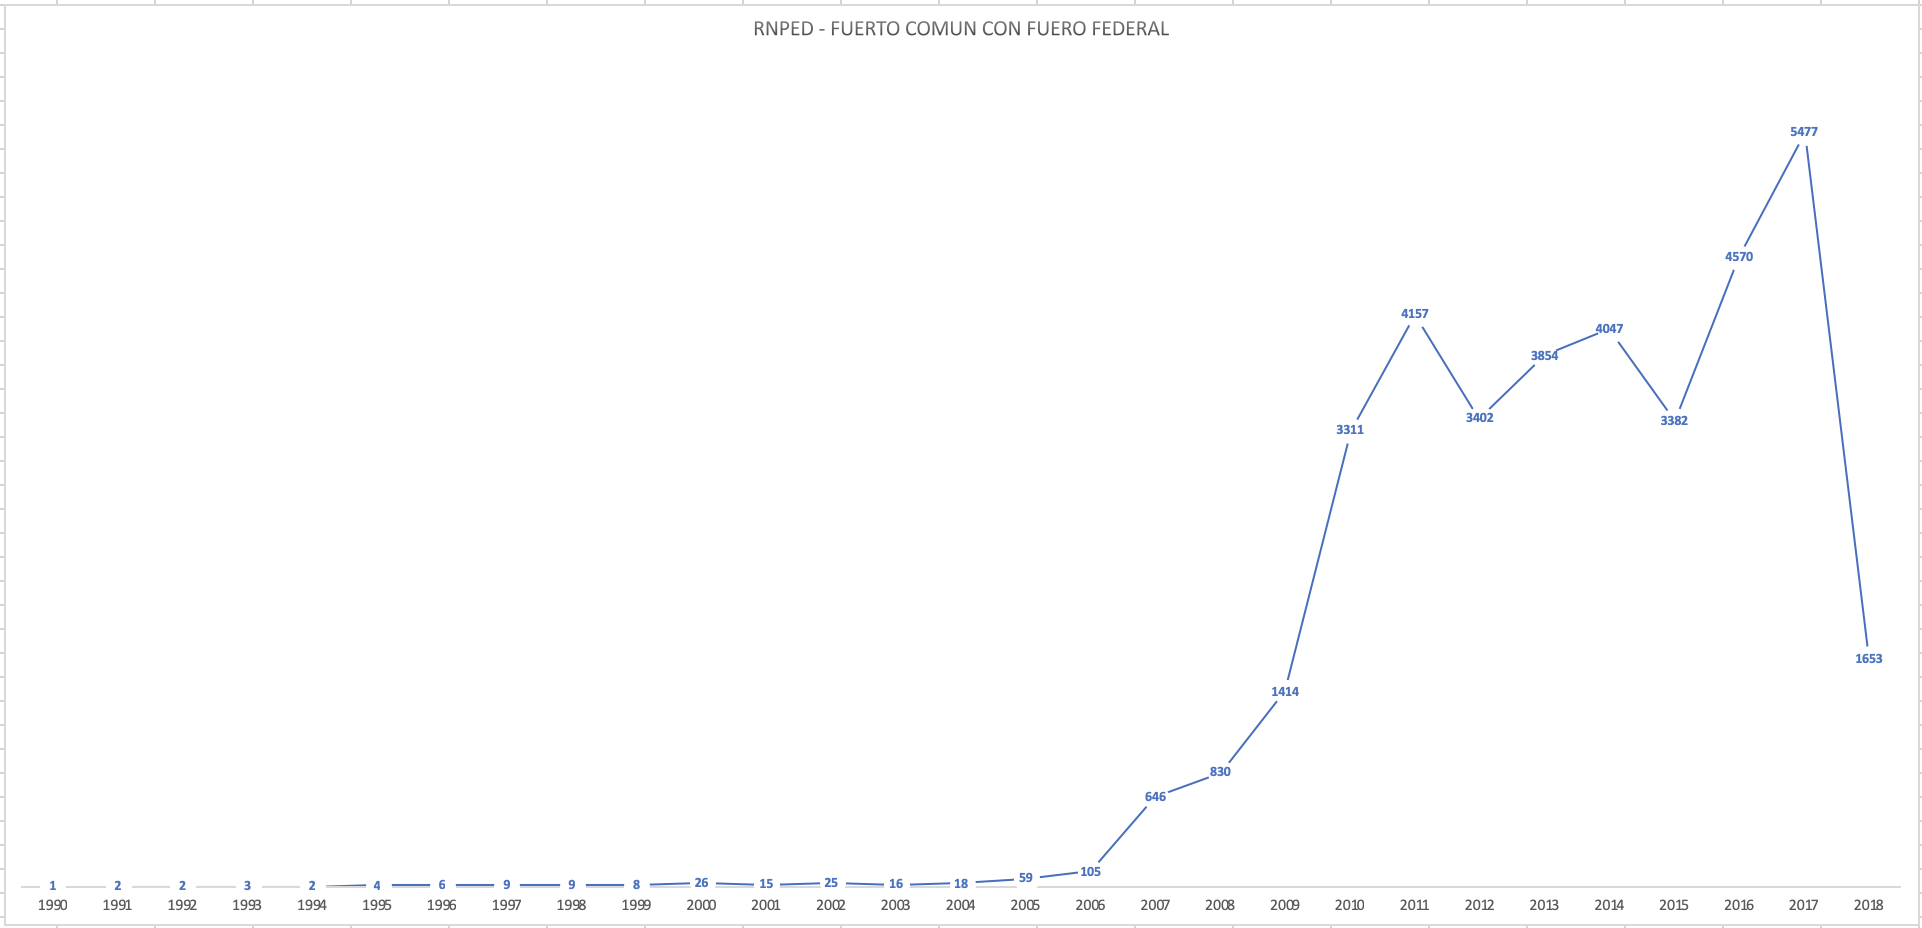
\includegraphics[width=5in]{imgs/fuerocomunYfuerofederal}
	  \caption{Estad\'istica Fuero Común y Fuero Federal}
\end{figure}

En la gr\'afina de la figura 3.3 podemos observar que entre 2006 y 2007 empieza un aumento repentino que alcanza su m\'animo punto en 2017 con 5477 personas desaparecidas. En 2018 se ve disminuido, sin embargo estos datos se ven influenciados debido a que del RNPED realizo su última fecha de corte el 30 de abril de 2018 (en el segundo trimestre del 2018), por motivos de delegar esta tarea a a la Comisión Nacional de Búsqueda de Personas, como lo informan en sus p\'agina:

\begin{quote}
\textit{Se informa que el Secretariado Ejecutivo del Sistema Nacional de Seguridad Pública realizó por última ocasión la actualización de las bases de datos del Registro Nacional de Datos de Personas Extraviadas o Desaparecidas (RNPD) del fuero común y fuero federal con corte al 30 de abril 2018.}
\end{quote}

\begin{quote}
\textit{
Cabe mencionar que corresponderá a la Comisión Nacional de Búsqueda de Personas la publicación de las subsecuentes bases de datos, de conformidad con la Ley General en materia de Desaparición Forzada de Personas, Desaparición cometida por Particulares y del Sistema Nacional de Búsqueda de Personas, publicado en el Diario Oficial en noviembre de 2017.}
\end{quote}


De esta manera no tenemos certeza de del número de desaparecidos en todo 2018 hasta que la Comisi\'on nacional de B\'usqueda de Personas haga p\'publicas sus bases de datos.

Por otra parte Roberto Cabrera Alfaro, Comisionado Nacional de B\'usqueda de Personas, presento su último informe el 17 de enero del 2019. Donde comunica que hasta esa fechas se tiene un registro de 40, 180 personas desaparecidas.

Si sumamos los datos por año desde 2007 seg\'un el RNPED y hacemos la diferencia con el informe de Roberto Cabrera Alfaro, de abril del 2018 a enero del 2019 nos da una cantidad estimada de 4985 desaparecidos en 2018. Lo cual nos habla de que la volumetria de desaparecidos se mantiene.

Para concluir podemos decir que la cifra de desaparecidos en M\'exico en la \'ultima decada (2009-2019) ha incrementado drasticamente y se ha vuelto un problema que necesita ser atendido.

\subsection{Homicidio en México 2018}

Según datos del Instituto Nacional de Estadística y Geografía, INEGI, en la gráfica de la figura 3.4, podemos observar los homicidios ocurridos en territorio nacional desde el año de 1990 a 2017.

Podemos observar que en 2007 llega a su punto más bajo en más de 15 años con 8867 homocidios, apartir de ahí incrementa en más de un 50\% respecto a 2007 llegando a su punto máximo en 2011 con 27213 homicidios (incrementando en más de un 300\% en tan solo 4 años) apartir de ahí baja hasta 2014 con 20010 homicidios, volviendo a subir, para bater record en 2017 con 31174 homicidios, la cifra más alta en más de 25 años, un dato realmente alarmante y que preocupa a la sociedad en general.

Lo anterior afecta directamente a la volumetria de personas desaparecidas, pues posiblemente éstas pertenezca al grupo de personas fallecidas sin identificar. Caso similar si una persona que se encontraba como desaparecida sea allada, pero en calidad de fallecida y disminuya la volumetria y las estadisticas de personas desaparecidas, más sin embargo lo que se busca es la integridad de las personas, es decir, que desaparezcan menos personas y las que se encuentran desaparecidas, se encuentren con vida.

\begin{figure}[bp!]
	\centering
	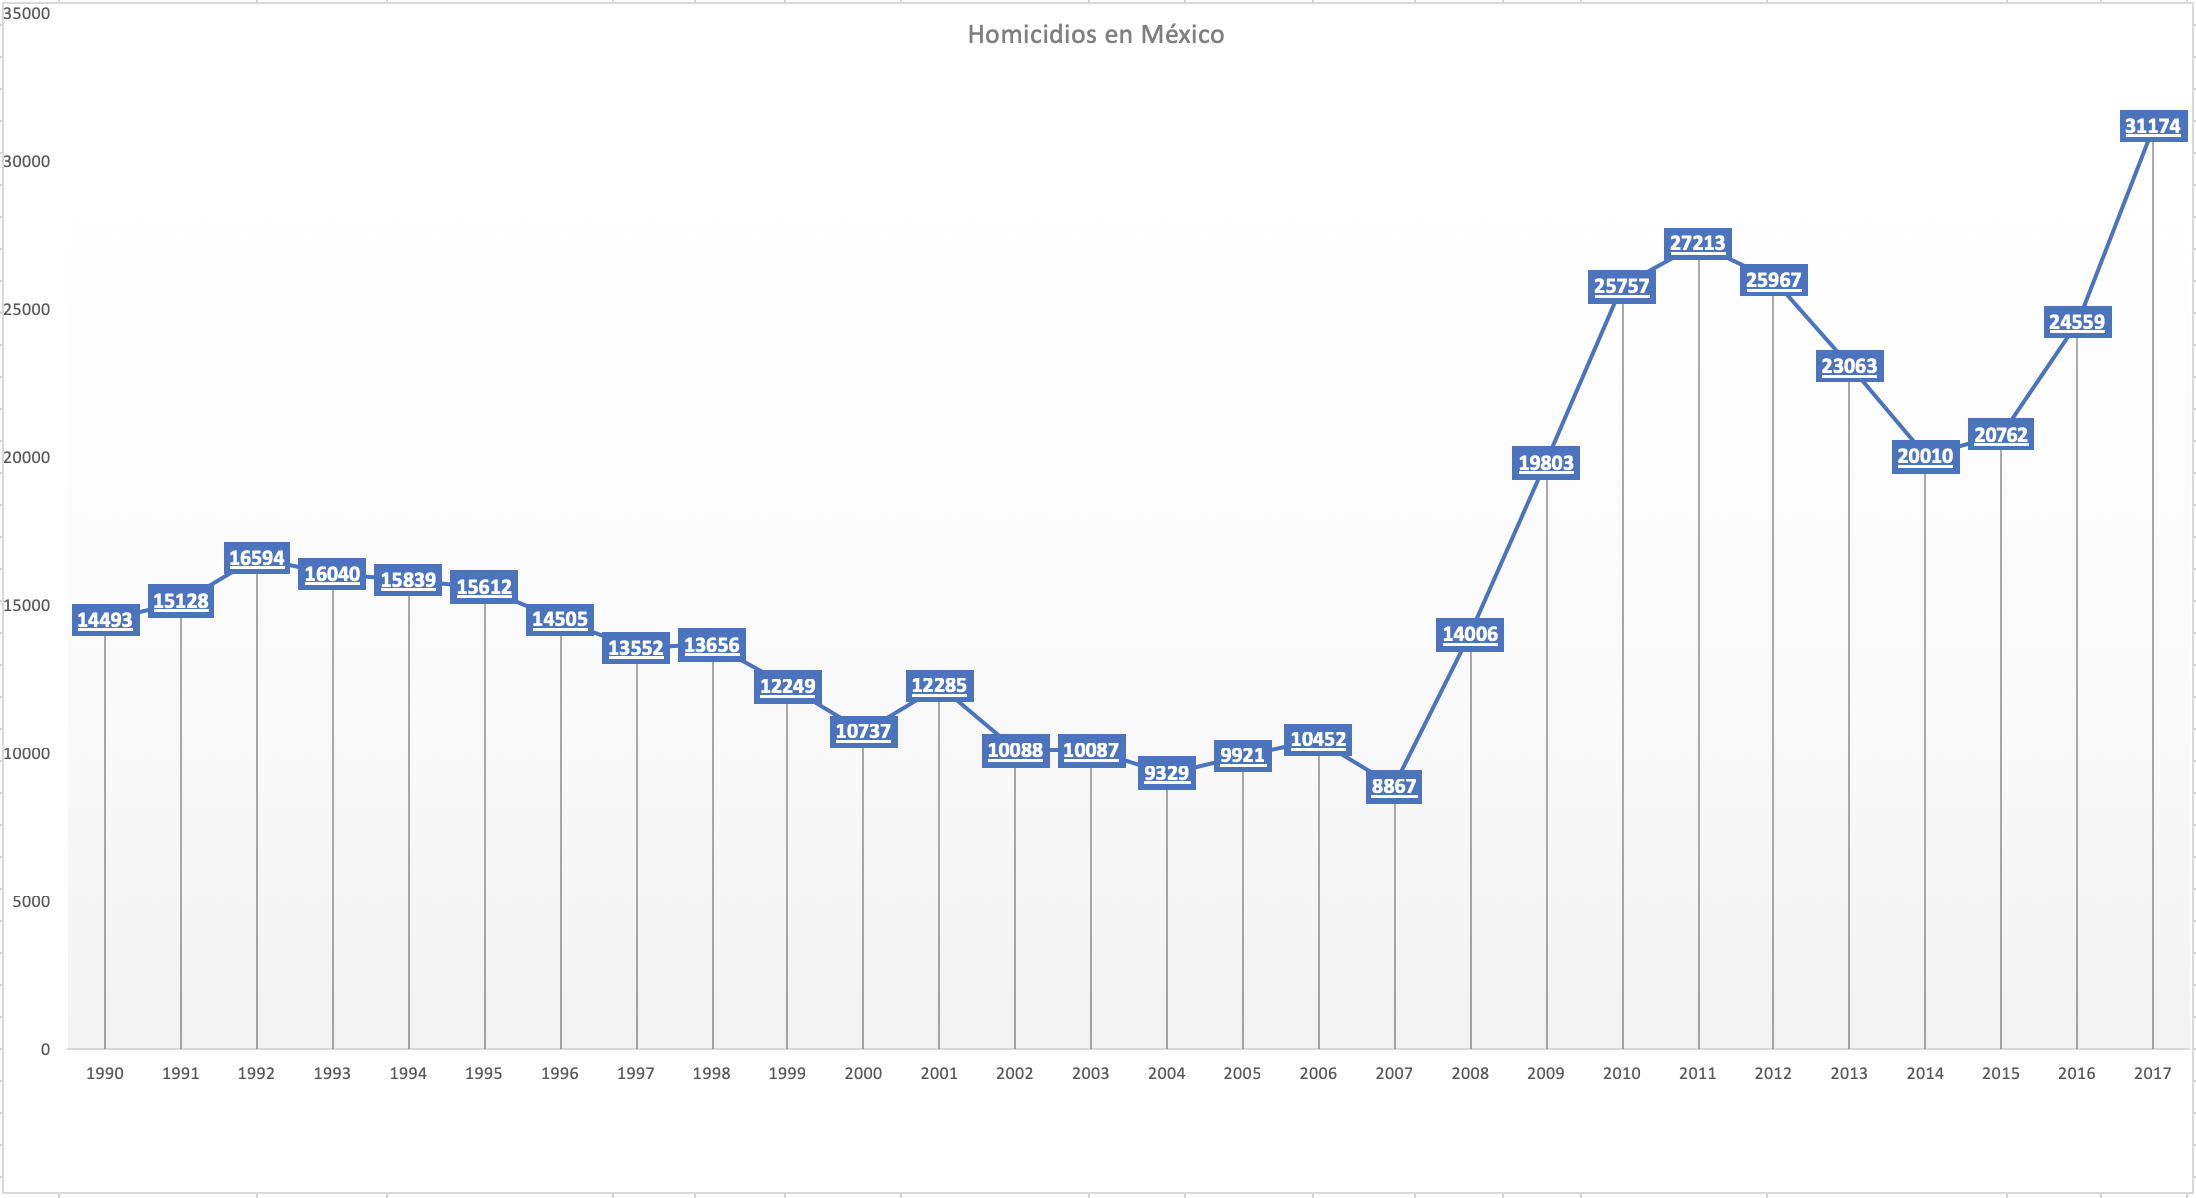
\includegraphics[width=5in]{imgs/homicidios}
	  \caption{Homicidios en México}
\end{figure}

%\newpage
\subsection{Percepción Sobre Seguridad Pública 2018}

Como su nombre lo indica el ENVIPE es la encuesta nacional sobre victimización y persepción sobre seguridad pública. 

Ofrece información referente al nivel de victimización y delincuencia, denuncia del delito, características de las víctimas de delito, los delitos y los daños causados, percepción sobre la inseguridad, desempeño institucional y la caracterización de los delitos en los hogares, entre otros.

Al mismo tiempo se da continuidad a la medición del grado de confianza social en las instituciones de seguridad pública y la percepción sobre su desempeño, los cambios en actividades y hábitos de las personas por temor al delito, la victimización del hogar y la victimización personal, así como a la identificación y medición de las actitudes y experiencias de las víctimas ante las instituciones de seguridad pública y de procuración de justicia.

La ENVIPE mide delitos que afectan de manera directa a las víctimas o a los hogares, tales como: Robo total de vehículo, Robo parcial de vehículo, Robo en casa habitación, Robo o asalto en calle o transporte público, Robo en forma distinta a las anteriores (como Carterismo, Allanamientos, Abigeato y Otros tipos de robo), Fraude, Extorsión, Amenazas verbales, Lesiones y Otros delitos distintos a los anteriores (como Secuestros, Delitos Sexuales y Otros delitos). 

Como podemos observar en 2017 el 29.74\% de la población en México ha sido victima de algún tipo de los delitos de los ya mencionados, redondeando 3 personas de cada 10. Si la taza de violencia sigue aumentando así podriamos decir que promediando las tazas de años anteriores (0.821857143p) para 2021, 1 de cada 3 personas seran victimas de algun tipo de delito de los anteriores mencionados. Lo cual tambien es un dato preocupante.

\begin{figure}[bp!]
	\centering
	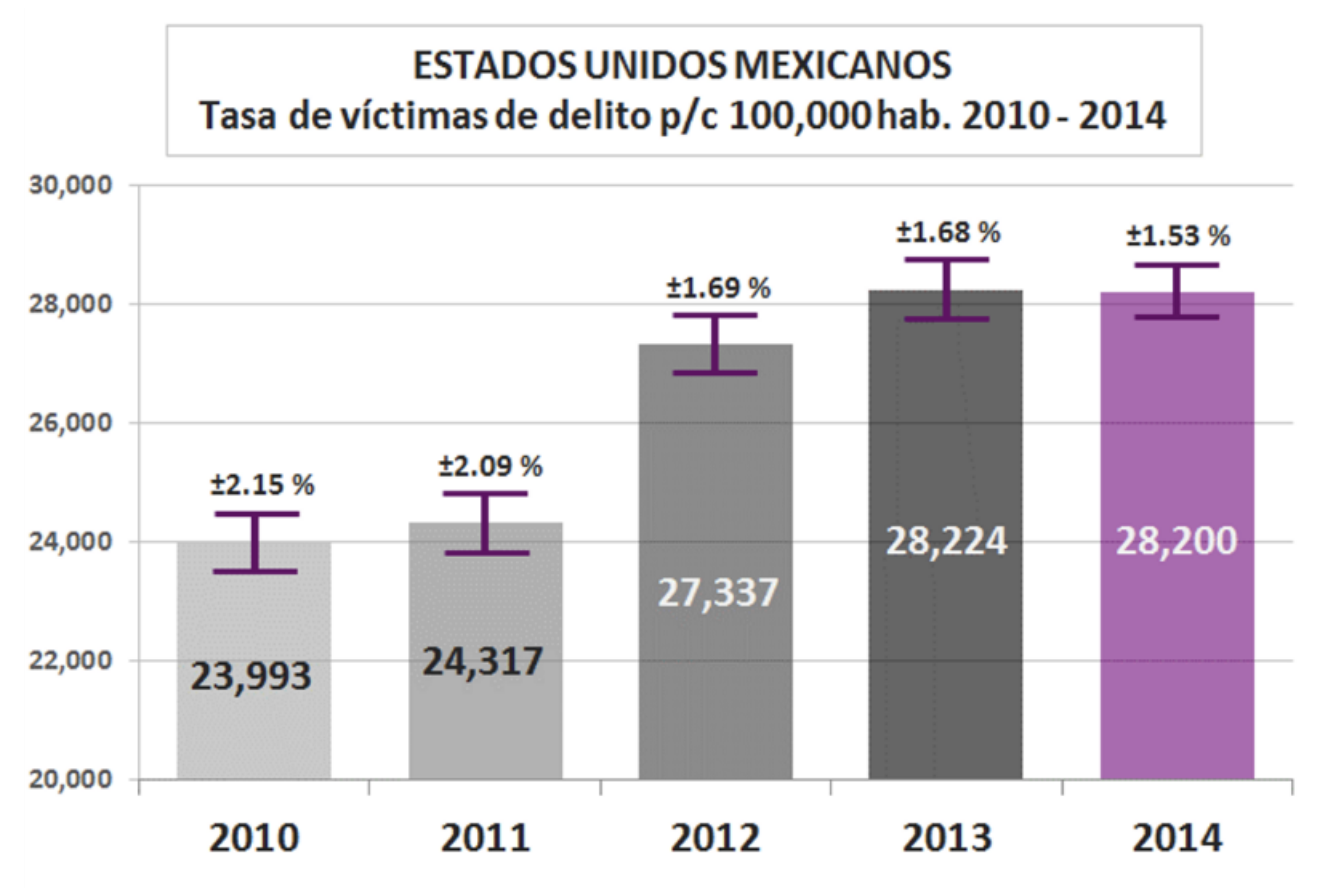
\includegraphics[width=5in]{imgs/envipe2010}
	  \caption{Tasa de v\'intimas de delito p/c 100, 000 habitantes. 2010-2014.}
\end{figure}

\begin{figure}[bp!]
	\centering
	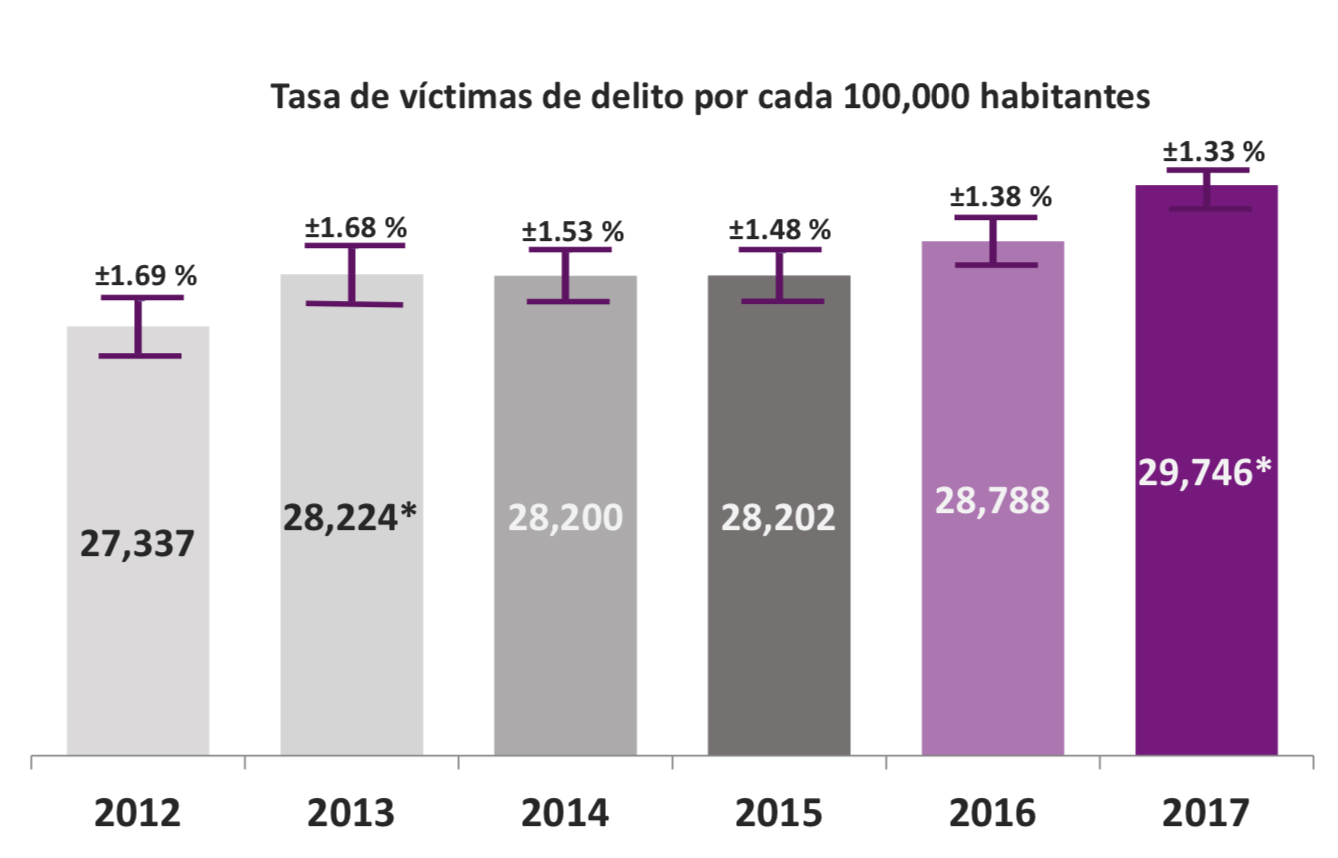
\includegraphics[width=5in]{imgs/envipe}
	  \caption{Tasa de v\'ictimas de delito por cada 100, 000 habitantes. 2012-2017.}
\end{figure}



\chapter{Marco Te\'orico}

\subsection{Computaci\'on Ubicua}

En 1991 Mark Weiser investigador en la Computer Science Laboratory en Xerox PARC publicaba un articulo llamado "La computadora para el siglo 21".

Para Weiser existen 3 etapas de la computación:

\begin{itemize}
    \item La era de los Mainframes o estaciones de trabajo.
    \item La era del computador personal.
    \item La era del computo ubicuo.
\end{itemize}

El computo ubicuo según Weiser, constituye la tercera ola de la computación. Básicamente es un entorno tecnológico en donde dispositivos de diferentes tamaños y funcionalidades, pueden conectarse y usarse en conjunto para manejar información, de forma que el hombre opera con mayor facilidad sus actividades del mundo cotidiano. Es decir, usar la tecnología a un nivel tan profundo que se desvanece en el tejido de la vida cotidiana, hasta que sea indistinguible.

Por lo tanto, estamos tratando de concebir una nueva forma de pensar acerca de las computadoras en el mundo, una que tenga en cuenta el entorno humano natural y permita que las mismas computadoras se desvanezcan en el fondo del ecosistema. Tal mezcla es una consecuencia fundamental no de la tecnología, sino de la psicología humana. Cuando las personas aprenden algo lo suficientemente bien, dejan de ser conscientes de ello.

La máquina multimedia de hoy, demanda la atención de la pantalla del ordenador, convirtiéndola en un foco de atención en lugar de permitir que se desvanezca en el fondo.

El sentido opuesto del computo ubicuo sería "realidad virtual" debido a que la realidad virtual se centra en un enorme aparato para simular el mundo, en lugar de mejorar de manera invisible el mundo, que ya existe.

Para explicar mejor el concepto de: "se desvance en el medio", podemos utiliza el ejemplo de "motores eléctricos dentro de un carro", están ahí al limpiar el parabrisas, al bloquear o desbloquear las puertas, pero no nos preocupamos de dónde están, sino que interactuamos de manera natural para realizar todas estas acciones. De esta manera el computo ubicuo busca que las computadoras sean invisibles.

Cientos de computadoras en una habitación suena intimidante, pero vendrán a ser invisibles a la conciencia común. La gente simplemente los usará inconscientemente para realizar tareas cotidianas.
El verdadero poder del concepto emerge de la interacción entre todos los dispositivos.

Hay más información disponible a nuestro alcance durante un paseo por el bosque que en cualquier sistema informático, sin embargo, la gente encuentra Un paseo entre árboles relajante y computadoras frustrantes. Máquinas que se adaptan al entorno humano, en lugar de obligar a los humanos a entrar en los suyos, hará que usar una computadora sea tan refrescante como pasear por el bosque.\cite{weiser}

\subsection{Movilidad inform\'atica}

Gracias a lo anterior podemos deducir que nos encontramos en la segunda era de la computación. La era del computador personal que a diferencia con la primera se caracteriza por la "movilidad física".

El usuario del entorno de computación móvil podrá acceder a datos, información u otros objetos lógicos desde cualquier dispositivo en cualquier red mientras esté en movimiento.\cite{asoke}

cliente servidor

Por lo tanto la "movilidad informatica" incluye cualquier dispositivo de computo fácilmente transportable y donde el usuario pueda realizar una tarea en movimiento o desde cualquier lugar en donde se encuentre. 

Usando un dispositivo de computación en una red pública (la web), o corporativa (información comercial) y espacios de información personal (registro médico, libreta de direcciones), etc. Lo que llamaremos aplicativos o aplicaciones.

Para llevarlo al siguiente nivel, el computo ubiquo, es necesario que el portador de la comunicación se extienda a través de medios inalámbricos y por cable. Es decir el dispositivo ubiquo compartira su información con el medio que lo rodea. Existirá tal cantidad de información que será necesario tratarla para sacar estadisticas o parametros que nos fáciliten la vida, incluso para que el dispositivo ubiquo pueda aprender de su propia información recolectada.

\subsection{Smarthphone}

\begin{figure}[bp!]
	\centering
	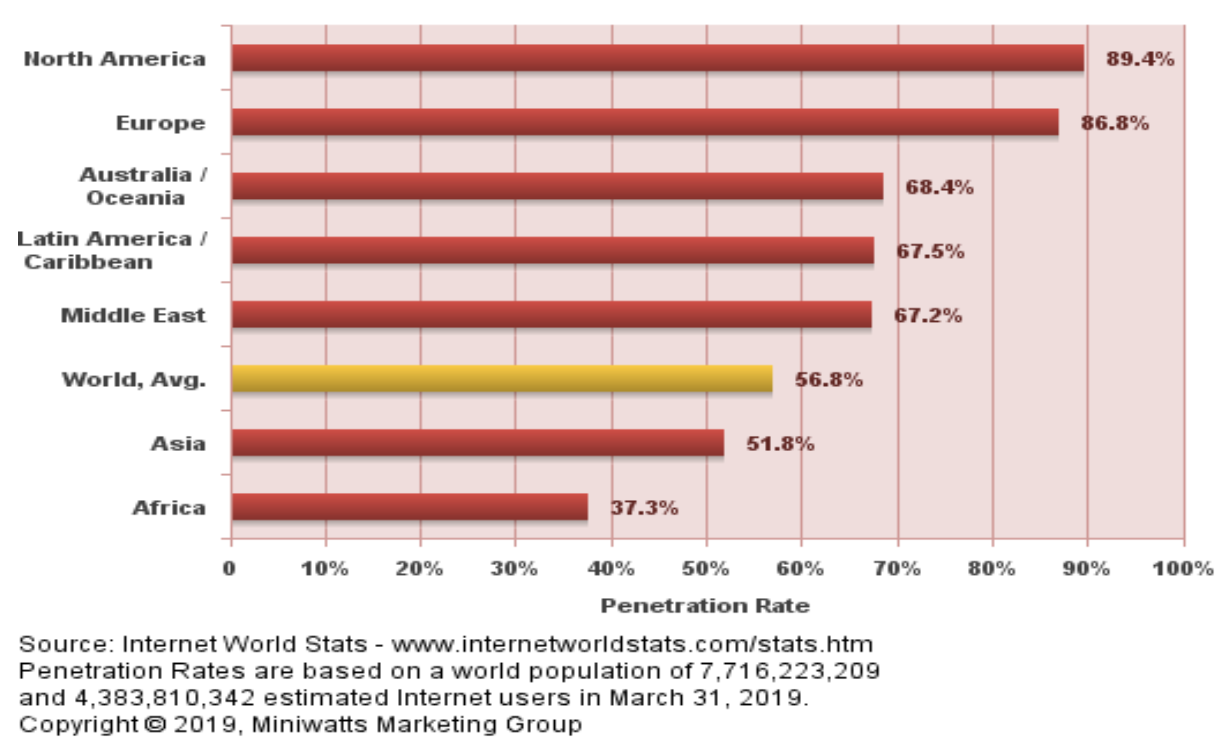
\includegraphics[width=5in]{imgs/internetPenetration19}
	  \caption{Internet World penetration rates by Geographic Regions - March, 2019}
\end{figure}

Actualmente la difusión de la tecnología móvil se ha visto ampliamente extendida principalmente a la penetración de internet en la sociedad \cite{internetPenetration}, así como la disminución en el costo de adquisición de los telefonos inteligentes o smarthphones. Sumado al acceso a la web a través de éstos. Ha detonado sin duda el uso habitual de telefonos inteligentes en nuestra sociedad actual.

Las ventajas de un telefono inteligente van más allá de poder acceder a internet y compartir información mieentras nos desplazamos. Cabe especificar que los telefonos inteligentes cuentan con diversos sensores integrados, como lo son: acelerómetros, giroscopio, sensor de huella, sensor dactilar, bluethoot, magnetómetro, receptor GPS, etc. Mismos que convirten al telefono inteligente en una navaja suiza y nos da un ecosistema fertil para un desarrollar infinidad de aplicativos. Tantos como nuestra imaginación.


\subsection{GPS}

Uno de los sensores principales con los que actualmente cuentan los telefonos intligentes es el receptor GPS. El Gps permite determinar la posición las 24 horas del día, en cualquier lugar del globo, bajo cualquier condición climatológica.\cite{latham}

A través del GPS podemos obtener: latitud, longitud, altitud del dispositivo. A su vez, a partir de estos datos podemos obtener información diversa, como: la velocidad de desplazamiento, la hora exacta, la distancia del dispositivo a un punto dado, si el dispositivo ha entrado a un area específica, si ha salido de un área en específica, principalmente.

\subsubsection{Arquitectura}

El sistema completo se compone de 3 elementos distintos denominados segmentos, los cuales son:

\begin{enumerate}
\item Segmento espacial: lo componen los satélites.
\item Segmento de control: lo componen las estaciones de control.
\item Segmento del usuario: lo componenlos receptores GPS.
\end{enumerate}
\newpage

\paragraph{Segmento espacial.}
 
	Está formado por una constelación de 24 satélites llamados SV (Space Vehicle). Circundan la tierra a 20.2000 km de altitud y forman 6 órbitas diferentes con 4 satélites cada una.
	Cada 24 horas (menos 4 minutos a causa del desplazamiento de la tierra al rededor del sol), se presenta exactamente en el mismo lugar y con la misma configuración respecto a los demás satélites.
	
	\begin{figure}[bp!]
	\centering
	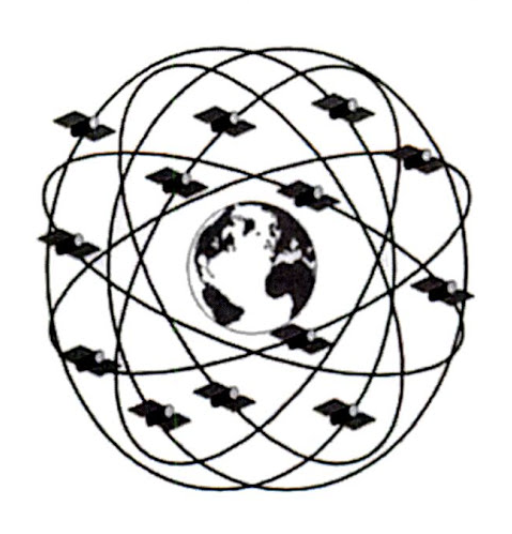
\includegraphics[width=3in]{imgs/24satelites}
	  \caption{La tecnología GPS se basa en un grupo de 24 satélites que emiten señales a la Tierra.}
\end{figure}

	Cada satelite envia un mensaje de navegación indicando su posición orbital así como la hora exacta de la emisión de dicho mensaje.
	
\paragraph{Segmento de control.}

	Se conforma por 5 estaciones de vigilacia y monitorización del sistema GPS, distribuidas al rededor del planeta, incluyendo una estación principal que asegura el correcto funcionamiento del sistema calculando las correcciones a aplicar.
	
	Las cinco estaciones se encuentran en las islas: Hawaii, Kwajalein (islas Marshall), Ascensión, Diego Garcia, en Colorado Springs. Su misión es captar todas las seáles emitidas por los satélites, acumular los mensajes recibidos y transmitir todas las informaciones recogidas a la estación principal.
	
\begin{figure}[bp!]
	\centering
	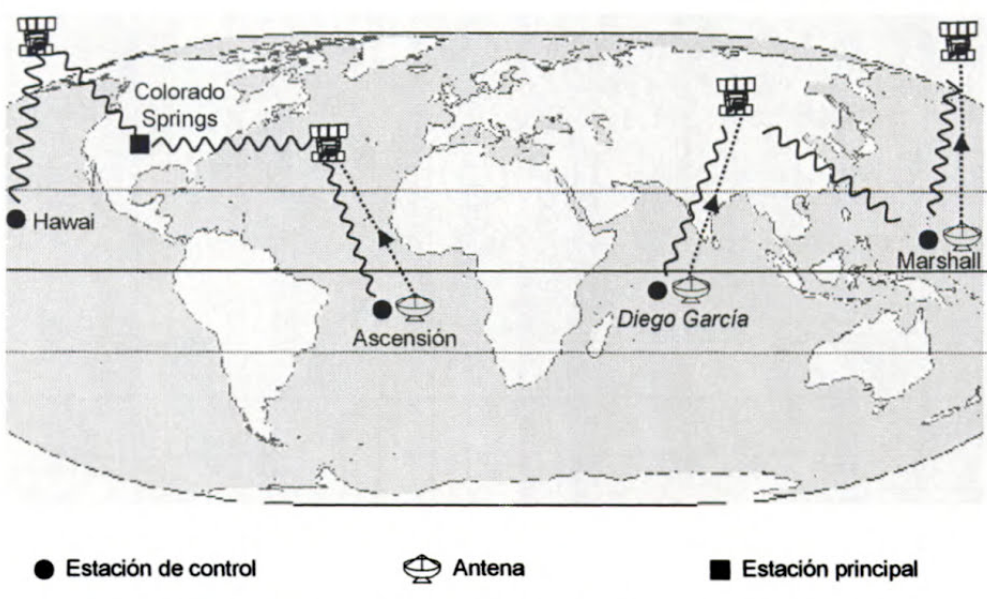
\includegraphics[width=5in]{imgs/estacionControl}
	  \caption{Estaciones de control.}
\end{figure}
	
\paragraph{Segmento del usuario.}

	Comprende la antena de recepción y el receptor (microprocesador) GPS. Podemos obtener información sobre posición, velocidad, ruta, hora y fecha.

\subsubsection{Servicio}

Existen dos tipos de servicio que brinda el sistema de posicionamiento global, uno público SPS (servicio de posicionamiento estándar) destinado a usuarios civiles en una sola frecuencia. El otro tipo de servicio es privado el PPS (servicio de posicionamiento preciso) este, está reservado para uso exclusivo del ejercito de USA.

El primero (SPS) está degradado con propósito de proteger la seguridad USA, la degradación consiste en una pequeña modificación del valor del reloj del satélite con ayuda de un generador pseudoaleatorio. Con un error inferior a 100 mts en horizontal y 156 mts en vertical, así como la hora con una precisión de 340 nanosegundos. El ejercito de USA puede modificar la degradación en caso de amenaza o un posible caso de guerra.

Por otro lado el PPS cuenta con un error inferior a los 21 mtrs en horizontal, de 27.7 mtrs en vertical y la hora con una precisión de 100 nanosegundos.



%\include{capitulo2}
%\include{capitulo3}
%\include{conclu}

%\appendix
%% Cap'itulos incluidos despues del comando \appendix aparecen como ap'endices
%% de la tesis.
%\include{apendiceA}
%\include{apendiceB}
%\include{apendiceC}

%% Incluir la bibliograf'ia. Mirar el archivo "biblio.bib" para m'as detales
%% y un ejemplo.

%\bibliography{biblio}
%\begin{thebibliography}{X}
%\bibitem{Baz} \textsc{Bazaraa, M.S., J.J. Jarvis} y \textsc{H.D. Sherali},
%\textit{Programacion lineal y flujo en redes}, segunda edicion,
%Limusa, M\'exico, DF, 2004.
%\bibitem{Dan} \textsc{Dantzig, G.B.} y \textsc{P. Wolfe},
%<<Decomposition principle for linear programs>>,
%\textit{Operations Research}, \textbf{8}, pags. 101--111, 1960. \end{thebibliography}


 
\medskip 
\bibliographystyle{unsrt}
\bibliography{biblio}


\end{document}